\section{To take away}
\begin{frame}
	\begin{columns}
		{\scriptsize
		\begin{column}{0.5\textwidth}
				\begin{alertblock}{Jet/SN interaction}
				\begin{itemize}
					\item A post-disruption expansion of the bow-shock, who covers the whole jet
					\item Provokes a jet speed local deceleration of $40\%$
					\item Results in a mass-load of $10^{-4}\,M_{\odot}\,{\rm yr}^{-1}$
					      over the interaction time scale 
				\end{itemize}
			\end{alertblock}
				\begin{exampleblock}{NT radiations}
					\begin{itemize}
						\item For sources closer or at 30Mpc, CTAO can make it in $\gamma$ 
						\item Chandra should easily detect the Synchrotron
						\item In radio (43Ghz) peak of $1\,{\rm MJy}$ at 200Mpc in Synchrotron
					\end{itemize}
				\end{exampleblock}
		\end{column}
			\hspace{-.5cm}
		\begin{column}{0.5\textwidth}
			\begin{block}{Longo et al. In prep}
				\begin{itemize}
					\item FRIs deceleration model (Perucho 2020)
					\item Stars entering the jet through the jet/ISM shear layer
					\item Trigger mixing between the ISM and the jet 
					\item Possible to apply the non thermal calculations to the shocked jet material
				\end{itemize}
			\end{block}
			\centering
			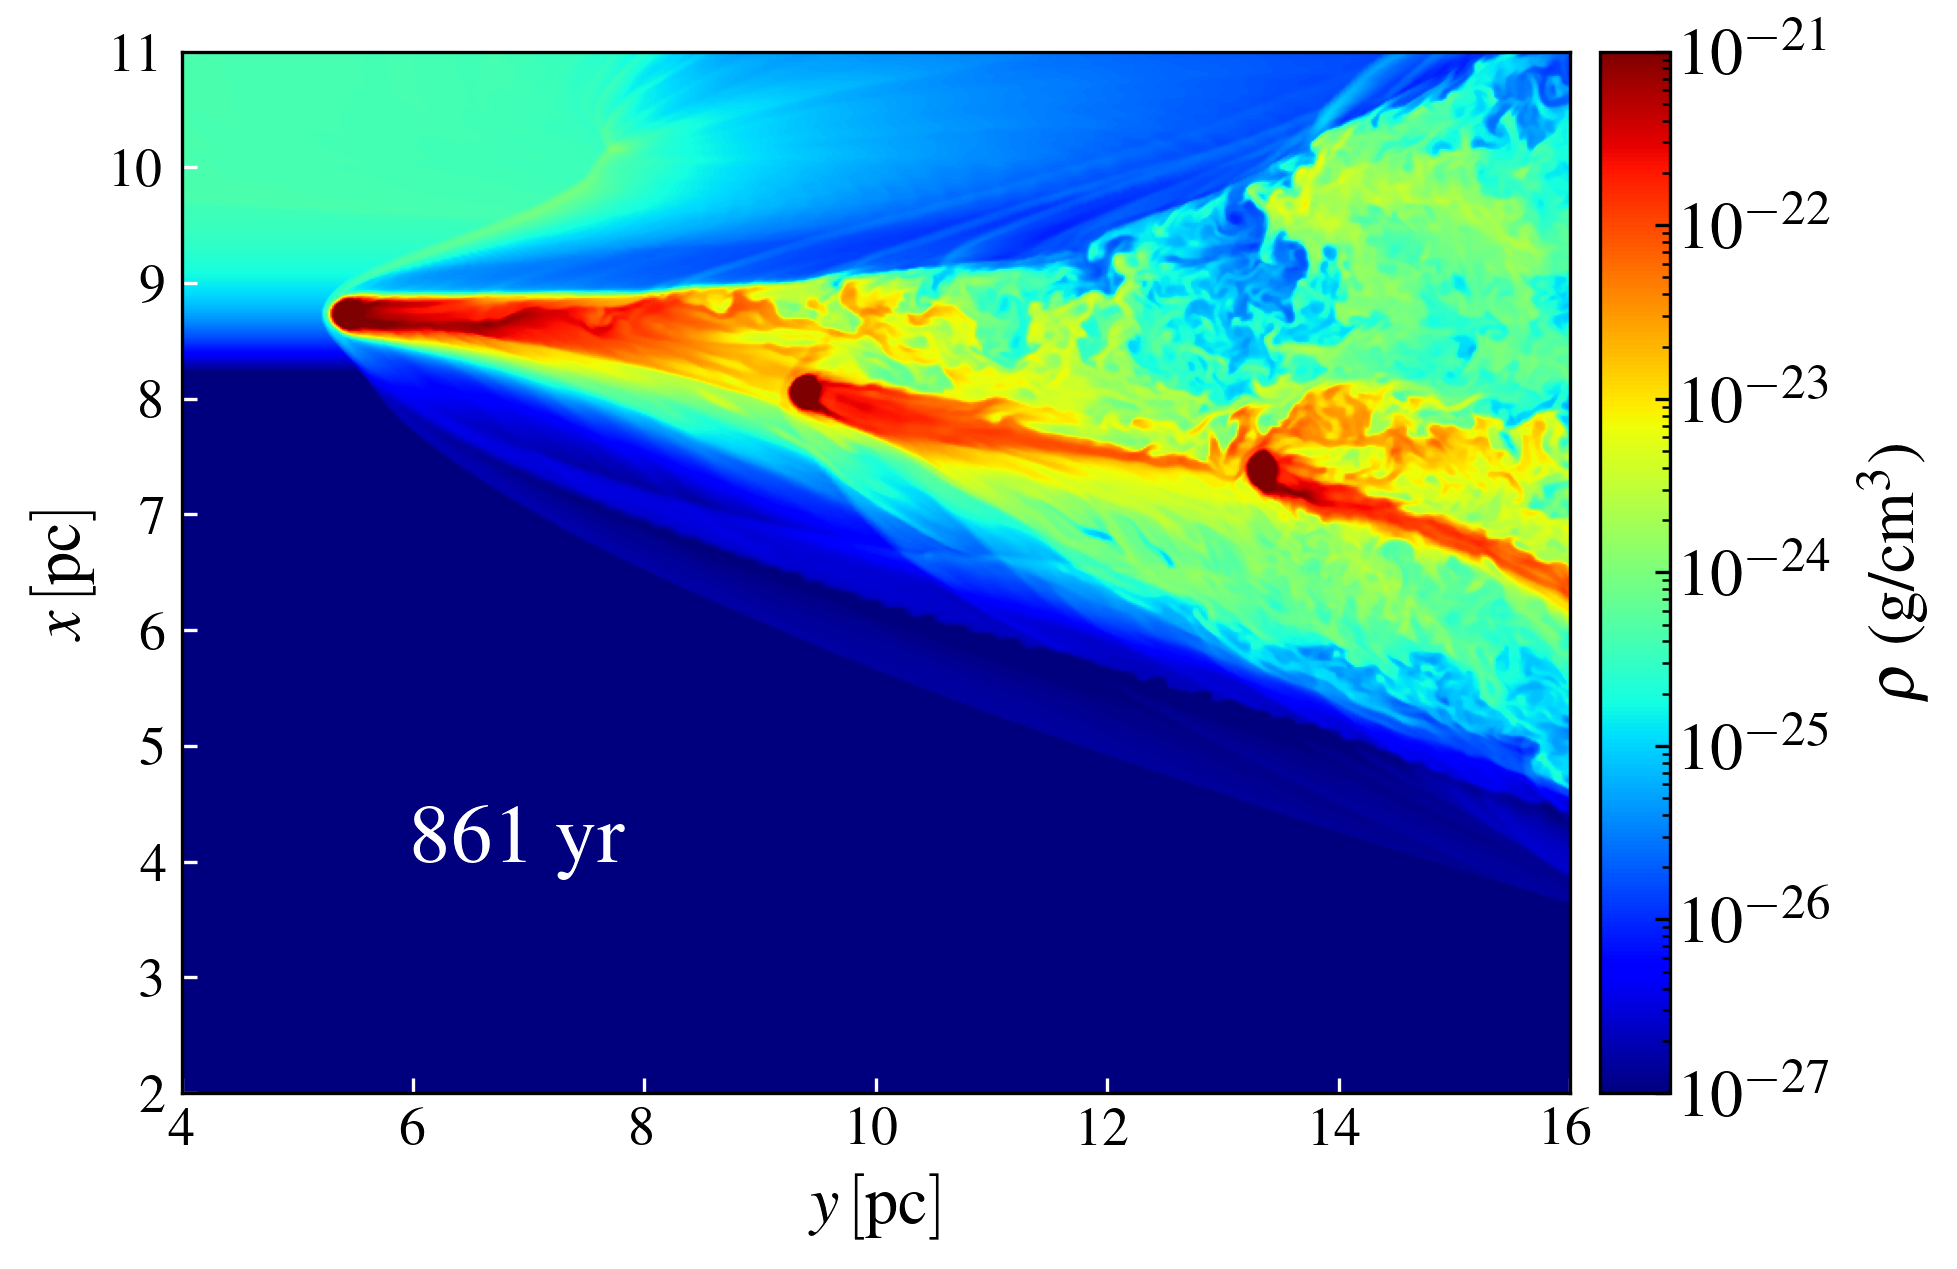
\includegraphics[width=\textwidth]{images/jbs3_130.png}
		\end{column}}
	\end{columns}
\end{frame}

\begin{frame}{}
	\centering
	\Huge{\textbf{Thank you}}
\end{frame}
